\Chapter{Implementáció}
A fejezet olyan problémák leírását tartalmazza, amiket a program írása során meg kellett oldanom. Nem Java stílusú LaTeX kódrészleteket tartalmaz, hanem beszúrt képeket a kész kódról.

\Section{Adattárolás}
Az adatok Firebase nevű felhőalapú adatbázisban kerülnek tárolásra, így az alkalmazás megfelelő működéséhez szükséges van internetkapcsolatra.
\\Az alkalmazást át kellett alakítanom Maven project-re, hogy a Firebase adatbázis driver-éhez hozzá tudjak férni, majd az API segítségével kapcsolatba tudjak lépni az adatbázissal.
\vspace{5pt}\\Az adatbázis interneten keresztül érhető el a \textit{https://console.firebase.google.com} címen. Az általam megadott e-mail címmel és jelszóval lehetséges a belépés.
\vspace{5pt}\\A Firebase ahhoz, hogy biztosítsa a mozgásban lévő adatainak biztonságát HTTPS protokollt használ, nyugvó adatait pedig titkosítja.

\Section{Grafikus Felhasználói Felület (GUI)}
A felhasználói felületet Java Swing használatával készítettem. A Swing egy GUI widget toolkit. Widget-ek alatt olyan grafikus elemeket értünk, mint gombok, szövegdobozok, listák, legördülő menük, stb...
\\A Swing egy régi technológia, viszont rengeteg alkalmazás használja. A Java GUI készítésre létrehoztak egy modernebb függvénykönyvtárat, ami a Swing-re épül, a JavaFX-et.
\\Kevésbé használt, mint a Swing, valószínűleg azért, mivel az alkalmazások nagy része Swing-ben készült, nincs szükség JavaFX-szé való konvertálásra. Új Java GUI-k írására valószínűnek tartom, hogy inkább JavaFX-et használnak.
\vspace{10pt}\\Azért választottam a Swing-et a JavaFX helyett, mert már dolgoztam a könyvtárral, míg a JavaFX-et egyáltalán nem ismertem, így azt gondoltam, hogy egyszerűbb dolgom lesz.
\\Hamar rá kellett jönnöm, hogy nem lesz olyan egyszerű dolgom, mint amire számítottam, de ettől függetlenül maradtam a Swing használata mellett. A widget-ek kinézetének megváltoztatására nem minden funkció elérhető, így nagyon sok időt kellett a szülő osztályok értelmezésével. Pár példa:
\vspace{5pt}\\A JButton widget egy gomb, amire lehet szöveget írni. Ha megnyomjuk a gombot, akkor megváltozik a színe, amíg el nem engedjük az egérgombot- Ezt a színt közvetlenül egy metódussal nem lehet megváltoztatni.
\\Gomb funkcióját JLabel widget-ek töltik ki, mert ezeknél könnyedén el lehetett érni, hogy gombnyomásra az általam megadott színűvé változzanak. Semmi hátrányom nem keletkezett abból, hogy JLabel-t használtam JButton helyett.
A jegyzetek és lapok listája is JList widget. A görgő kinézetét nem lehet közvetlenül megváltoztatni, így meg kellett keresnem hol kerül kirajzolásra a görgő, megkeresni hogy milyen metódusokat használ, majd azokat felülírni. 

\begin{figure}[h]
	\centering
	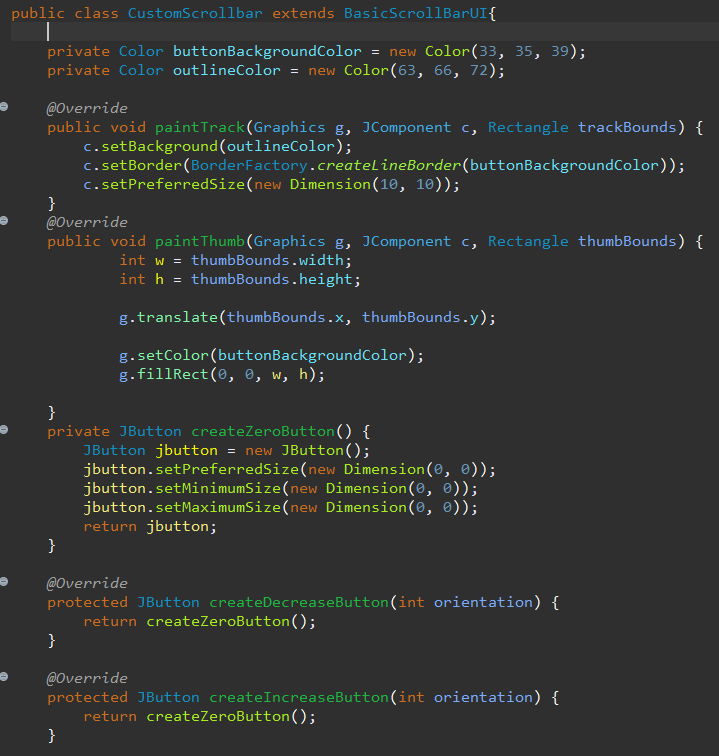
\includegraphics[scale=0.4]{images/code_1.png}
	\caption{Egyedi görgő rajzolásának megoldása}
	\label{fig:code_scrollbar}
\end{figure}
\vspace{5pt}\noindent A lista elemeinek sem lehetett egyszerűen megváltoztatni a kinézetét, méretét, keret színét, stb.. Ezeket is a görgőhöz hasonló módon kellett megkeresnem.
\begin{figure}[h]
	\centering
	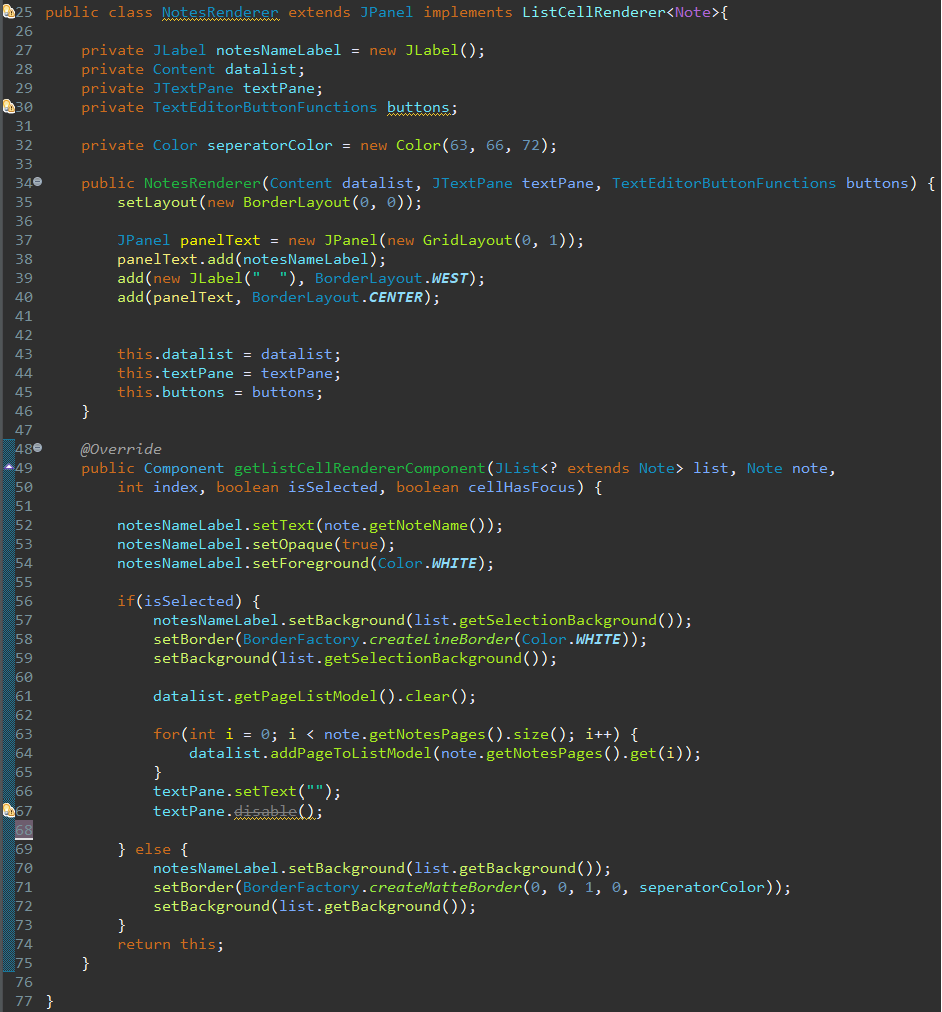
\includegraphics[scale=0.3]{images/code_2.png}
	\caption{Listaelemek egyedi megjelenése, kijelölés egyedi megjelenése.}
	\label{fig:code_list_item}
\end{figure}
\vspace{10pt}\noindent \\ A program írása szempontjából a legnehezebb rész számomra a GUI elkészítése volt. Nagyon sok dolog nem érhető el Swing-ben közvetlenül, amire az ember logikusnak hinné, hogy elérhető.
\\Próbáltam egy modernebb felületet létrehozni, de ez csak a közvetlenül elérhető metódusok használatával nem lehetséges. Ha csak azokat használjuk, akkor egy 'régi' megjelenésű szoftvert tudunk csak készíteni.

\subsection{Titkosítás}

Az adatok az applikáción belül kerülnek titkosításra, még az adatbázisba való töltés előtt.
\vspace{5pt} \\ Először egy struktúrált XML dokumentumba rendezi az alkalmazás az adatokat, ezután az XML dokumentum byte-jait AES algoritmus alkalmazásával titkosítja. 
\vspace{5pt} \\ Az adatbázisba a titkosított XML dokumentum kerül feltöltésre.
\vspace{15pt} \\Adatok titkosítása majd adatbázisba küldése két esetben lehetséges. Vagy a bal felső sarokban lévő mentés gombra kattintva (ctrl+s), vagy az alkalmazás bezárása előtti automatikus mentés során, feltéve ha van éppen internetkapcsolat.

\subsection{Visszafejtés}
Az adatok visszafejtéséhez ugyanazt a szimmetrikus kulcsot használja az alkalmazás, mint a titkosításhoz.
\vspace{5pt} \\ Visszafejtés csak egyszer történik, az applikáció indításakor, amikor lekéri az alkalmazás a titkosított XML dokumentumot az adatbázisból.


\subsection{Kulcskezelés}
A titkosításhoz és visszafejtéshez egy random generált, 256 bit-es AES titkosítási kulcsot alkalmaztam és ahogy a teszt-alkalmazásokban, úgy itt is a javax.crypto függvénykönyvtárat használtam.
\vspace{5pt} \\ Ez a titkosítási kulcs egy .jks, azaz java keystore fájl-ban kerül tárolásra. A fájl tartalma jelszóval védett.
\\Az alkalmazás (első) indításával jön létre ez a fájl az adott eszközön.



